\chapter{Testing and Evaluation}
\label{chap:testing}

Evaluation of the platform proceeds against the requirements from Chapter~\ref{chap:requirements}.
Section~\ref{sec:test-approach} outlines the testing strategy used. Requirements
are assessed one by one in Section~\ref{sec:test-requirements}. Performance and scalability
considerations follow in Section~\ref{sec:test-performance}, and Section~\ref{sec:test-deployment}
covers the CZU deployment and the path to eLTER adoption.

%% ----------------------------------------------------------------
\section{Testing Approach}
\label{sec:test-approach}
%% ----------------------------------------------------------------

Testing operates at three levels: automated unit and integration tests for the
data platform backend and frontend, automated tests inherited from the upstream
\texttt{tsm-orchestration} codebase, and manual end-to-end verification of the full
deployment.

\subsection{Backend Test Suite}
\label{sec:test-approach-backend}

A pytest-based test suite covering 804~test
functions across 43~test files is included with the data platform backend, organized into five directories:
\texttt{test\_api/} (endpoint-level tests), \texttt{test\_services/} (business-logic tests),
\texttt{test\_core/} (middleware, security, and exception handling), \texttt{test\_schemas/}
(Pydantic model validation), and \texttt{test\_tasks/} (Celery background tasks).

Test fixtures are defined in \texttt{conftest.py}. A \texttt{mock\_db\_session} fixture
provides a \texttt{MagicMock(spec=Session)} for SQLAlchemy interactions. The \texttt{client}
fixture creates a FastAPI \texttt{TestClient} with dependency overrides that inject the mocked
database session and an authenticated admin user, enabling endpoint tests to run without a
real database or Keycloak instance. An autouse \texttt{disable\_seeding} fixture prevents
the application from running database initialization at startup.

Custom pytest markers (\texttt{api}, \texttt{services}, \texttt{core}, \texttt{v1}) are
assigned automatically based on the test file's directory, enabling selective test execution.
By default, \texttt{pytest.ini} excludes tests marked as
\texttt{integration}, which require a live PostgreSQL instance.

Coverage is measured with \texttt{pytest-cov} against the \texttt{app/} package. The
largest test files target the most critical business logic: the TimeIO database service
(152~tests covering schema management and observation queries), the RBAC permission resolver
(76~tests covering role inheritance, batch resolution, and group-based authorization),
and the alert evaluator (69~tests covering all operators, deduplication, sensor data
evaluation, and QA/QC rule evaluation).

A Locust\footnote{Locust load testing tool: \url{https://locust.io/}}-based load testing suite is included in \texttt{tests/load/locustfile.py}. It
simulates authenticated users performing weighted API operations (project listing, sensor
queries, observation retrieval) against a running instance. The load test can be scaled
via \texttt{docker-compose.loadtest.yml}, which supports multiple Locust worker containers.

\subsection{Frontend Test Suite}
\label{sec:test-approach-frontend}

The frontend includes 96~test cases in 13~files under \texttt{frontend/\_\_tests\_\_/},
executed with Vitest\footnote{Vitest testing framework: \url{https://vitest.dev/}} and React Testing Library against a jsdom environment. The tests cover
the API interceptor (authentication header injection and error handling), React~Query hook
factories (query key generation, mutation lifecycle), and selected component rendering
(project cards). The Vitest configuration uses the \texttt{@vitejs/plugin-react} plugin
and resolves import aliases through the same path mapping used in production.

\subsection{TSM Orchestration Tests}
\label{sec:test-approach-tsm}

Upstream \texttt{tsm-orchestration} contains 131~test functions covering
parser implementations (CSV, JSON), worker scripts (file ingest, crontab setup), external
API syncers (DWD, TTN, Bosch, T-Systems, UBA), Grafana API integration, and cryptographic
utilities. These tests were inherited with the fork and continue to pass against the
modified codebase.

\subsection{Manual End-to-End Verification}
\label{sec:test-approach-e2e}

Full-stack scenarios are verified manually against a running deployment. A primary
verification path traces the complete Thing lifecycle: sensor creation through the portal,
infrastructure provisioning by TSM workers (observable through container logs and database
schema creation), data ingestion via MQTT or CSV upload, observation availability through
the FROST-Server STA endpoint, and time-series rendering in the portal charts. The
\texttt{make check} target in the deployment layer automates the infrastructure-level
portion of this verification by probing container health, HTTP endpoint reachability, and
\texttt{@sync} variable consistency.

%% ----------------------------------------------------------------
\section{Evaluation Against CZU Requirements}
\label{sec:test-requirements}
%% ----------------------------------------------------------------

Each functional and non-functional requirement from Chapter~\ref{chap:requirements} is
evaluated below. Requirements are classified as \emph{fully met}, \emph{partially met},
or \emph{not met}, with evidence from the test suite, source code, or deployed system.

\subsection{Functional Requirements}
\label{sec:test-requirements-functional}

Table~\ref{tab:req-evaluation-fr} summarizes the evaluation of functional requirements.

\begin{landscape}
{\small
\begin{longtable}{l p{0.30\linewidth} l p{0.38\linewidth}}
  \caption{Functional requirements evaluation.}
  \label{tab:req-evaluation-fr} \\
  \textbf{ID} & \textbf{Requirement} & \textbf{Status} & \textbf{Evidence} \\
  \hline
  \endfirsthead
  \textbf{ID} & \textbf{Requirement} & \textbf{Status} & \textbf{Evidence} \\
  \hline
  \endhead
  FR-1  & MQTT real-time ingestion with per-Thing parsers
        & Fully met
        & mqtt-ingest worker; parser framework with 5~device-specific parsers;
          131~upstream tests pass. \\[3pt]
  FR-2  & CSV file upload ingestion
        & Fully met
        & file-ingest worker; 13~\texttt{test\_things.py} tests cover CSV upload
          endpoint. \\[3pt]
  FR-3  & External SFTP synchronization
        & Fully met
        & sync-extsftp worker; triggered by cron via MQTT. \\[3pt]
  FR-4  & External REST API synchronization
        & Fully met
        & sync-extapi worker; DWD, TTN, Bosch, T-Systems, UBA syncers;
          30~upstream syncer tests. \\[3pt]
  FR-5  & Custom parser and syncer script upload
        & Fully met
        & Dynamic loader fetches scripts from MinIO; AST-based validation blocks
          dangerous operations. \\[3pt]
  FR-6  & Sensor CRUD with parser and coordinate config
        & Fully met
        & 25~\texttt{test\_sms.py} tests; 31~\texttt{test\_orchestrator.py}
          tests. \\[3pt]
  FR-7  & Bulk sensor import from CSV template
        & Fully met
        & \texttt{BulkImportDialog} component; 6~\texttt{test\_bulk.py} tests
          with validation and authorization checks. \\[3pt]
  FR-8  & Sensor inactivity detection and alerting
        & Fully met
        & \texttt{MonitoringService}; 51~\texttt{test\_monitoring\_service.py}
          tests. \\[3pt]
  FR-9  & Reusable MQTT device types and CSV parsers
        & Fully met
        & SMS catalog endpoints; parser/device-type CRUD tested in
          \texttt{test\_sms.py}. \\[3pt]
  FR-10 & Project CRUD with sensor grouping
        & Fully met
        & 10~\texttt{test\_project\_service.py} tests;
          6~\texttt{test\_projects.py} endpoint tests. \\[3pt]
  FR-11 & Project member roles (owner/editor/viewer)
        & Fully met
        & Two-tier RBAC; 76~\texttt{test\_rbac\_service.py} tests cover role
          inheritance and batch resolution. \\[3pt]
  FR-12 & Per-project TimeIO schema provisioning
        & Fully met
        & \texttt{TimeIOOrchestrator}; 152~\texttt{test\_timeio\_db.py} tests
          cover schema management. \\[3pt]
  FR-13 & QA/QC test pipeline configuration
        & Fully met
        & QA/QC endpoints at project and SMS scope;
          \texttt{SensorQAQCSection} frontend component. \\[3pt]
  FR-14 & Automatic QA/QC on \texttt{data\_parsed} event
        & Fully met
        & run-qaqc worker subscribes to \texttt{data\_parsed} topic. \\[3pt]
  FR-15 & On-demand QA/QC triggering via API
        & Fully met
        & QA/QC service publishes to \texttt{data\_parsed} to trigger
          re-evaluation. \\[3pt]
  FR-16 & Interactive time-series charts
        & Fully met
        & \texttt{TimeSeriesChart} component with Recharts; zoom via
          \texttt{ReferenceArea} and \texttt{Brush}. \\[3pt]
  FR-17 & Interactive map with sensor markers and WMS overlay
        & Fully met
        & \texttt{ProjectMap} with MapLibre~GL; GeoServer WMS layer overlay;
          30-second auto-refresh. \\[3pt]
  FR-19 & CSV export of Observation data
        & Fully met
        & Export endpoint in \texttt{things.py} router. \\[3pt]
  FR-20 & OIDC authentication via Keycloak
        & Fully met
        & JWKS validation in \texttt{core/security.py}; 4~\texttt{test\_auth.py}
          tests; 7~\texttt{test\_keycloak\_service.py} tests. \\[3pt]
  FR-21 & Two-tier RBAC model
        & Fully met
        & \texttt{RBACService} with six-rule priority chain;
          76~permission tests. \\[3pt]
  FR-22 & Keycloak group management
        & Partially met
        & Group management decommissioned from portal; users manage groups
          via the Keycloak admin console directly. \\[3pt]
  FR-23 & Historical CSV data upload (up to 200~MB)
        & Fully met
        & \texttt{DataUploadModal} and \texttt{DatasetUploadModal} components;
          files stored in per-Thing MinIO bucket. \\[3pt]
  FR-24 & GeoJSON geospatial import (up to 200~MB)
        & Fully met
        & Bulk import endpoint; 6~\texttt{test\_bulk.py} tests cover streaming
          and validation. \\[3pt]
  FR-25 & Multilingual UI (EN, CS, SK)
        & Fully met
        & Zustand-persisted locale store; typed dictionary files for all three
          languages. \\
\end{longtable}
}
\end{landscape}

\begin{landscape}
\subsection{Non-Functional Requirements}
\label{sec:test-requirements-nonfunctional}

Table~\ref{tab:req-evaluation-nfr} summarizes the evaluation of non-functional requirements.

{\small
\begin{longtable}{l p{0.30\linewidth} l p{0.38\linewidth}}
  \caption{Non-functional requirements evaluation.}
  \label{tab:req-evaluation-nfr} \\
  \textbf{ID} & \textbf{Requirement} & \textbf{Status} & \textbf{Evidence} \\
  \hline
  \endfirsthead
  \textbf{ID} & \textbf{Requirement} & \textbf{Status} & \textbf{Evidence} \\
  \hline
  \endhead
  NFR-1 & Containerized deployment (Docker + Podman)
        & Fully met
        & The deployment layer supports both runtimes; \texttt{podman\_prep.py}
          applies seven transformations. \\[3pt]
  NFR-2 & OGC STA compliance
        & Partially met
        & FROST-Server serves STA queries; local STA views provide entity data
          but stub views for \texttt{SENSORS}, \texttt{OBS\_PROPERTIES}, and
          \texttt{FEATURES\_OF\_INTEREST} return empty results. \\[3pt]
  NFR-3 & OIDC standards compliance
        & Fully met
        & RS256 JWKS validation with one-hour TTL cache; multi-issuer support;
          \texttt{asyncio.Lock} for concurrent refresh. \\[3pt]
  NFR-4 & Modular extensibility
        & Fully met
        & Dynamic parser loading from MinIO; runtime-uploadable syncer
          scripts. \\[3pt]
  NFR-5 & Security (script sandboxing, rate limiting, encryption)
        & Fully met
        & AST-based script validation; SlowAPI rate limiting; Fernet credential
          encryption; 10~\texttt{test\_crypto\_utils.py} tests. \\[3pt]
  NFR-6 & Maintainability (migrations, OpenAPI docs)
        & Fully met
        & Four Alembic migrations for \texttt{water\_dp} schema; Flyway for
          TSM; OpenAPI docs generated automatically by FastAPI. \\[3pt]
  NFR-7 & eLTER interoperability alignment
        & Partially met
        & STA-based data access satisfies (a); Keycloak OIDC supports federation
          with eLTER~LogIn~(b); data model is extensible for DEIMS-SDR and
          EnvThes~(c); per-site Docker~Compose deployment preserves
          autonomy~(d). No eLTER-specific metadata schemas or vocabulary
          bindings implemented yet. \\[3pt]
  NFR-8 & Unified deployment via single config
        & Fully met
        & Single \texttt{.env} with symlinks; \texttt{make up} deploys the
          full stack; \texttt{make check} validates health. \\
\end{longtable}
}
\end{landscape}

\subsection{Gap Analysis Closure}
\label{sec:test-requirements-gaps}

Table~\ref{tab:gap-closure} maps the eleven gaps identified in
Section~\ref{sec:req-gap} to their resolution status.

\begin{longtable}{l l p{0.70\textwidth}}
  \caption{Gap analysis closure.}
  \label{tab:gap-closure} \\
  \textbf{Gap} & \textbf{Status} & \textbf{Resolution} \\
  \hline
  \endfirsthead
  \textbf{Gap} & \textbf{Status} & \textbf{Resolution} \\
  \hline
  \endhead
  G-1  & Resolved & Project model with member roles and sensor assignment
         implemented in the \texttt{water\_dp} schema. \\[3pt]
  G-2  & Resolved & Next.js portal with time-series charts, maps, alerts,
         QA/QC, and sensor management. \\[3pt]
  G-3  & Resolved & GeoServer integration with REST~API layer management and
         MapLibre~GL WMS overlay. \\[3pt]
  G-4  & Resolved & Nine local STA views replace the SMS-dependent views;
         FROST-Server starts and serves valid STA responses. \\[3pt]
  G-5  & Resolved & The data platform replaces the non-functional SMS with
         sensor management endpoints and the \texttt{TimeIOOrchestrator}. \\[3pt]
  G-6  & Resolved & Alert evaluation system with sensor threshold, QA/QC, and
         inactivity rules; MQTT-triggered processing. \\[3pt]
  G-7  & Resolved & The deployment layer with Compose multi-file merge,
         \texttt{@sync} validation, and Makefile interface. \\[3pt]
  G-8  & Resolved & \texttt{podman\_prep.py} generates Podman-compatible Compose
         files; rootless-specific UID/GID and network fixes applied. \\[3pt]
  G-9  & Resolved & Three locale files (EN, CS, SK) with Zustand-persisted
         language switching. \\[3pt]
  G-10 & Resolved & \texttt{TimeIOOrchestrator} generates MQTT configuration
         messages compatible with the ingestion pipeline. \\[3pt]
  G-11 & Resolved & SMS catalog endpoints for parser and device-type CRUD;
         dynamic parser loading from MinIO. \\
\end{longtable}

All eleven gaps from the baseline analysis are resolved. Two non-functional requirements
(NFR-2 and NFR-7) remain partially met: NFR-2 due to the stub STA entity views that
return empty results for entities without a local equivalent, and NFR-7 due to the
absence of eLTER-specific metadata schemas, which are planned as future work.

%% ----------------------------------------------------------------
\section{Performance and Scalability Considerations}
\label{sec:test-performance}
%% ----------------------------------------------------------------

To validate that the platform meets its response-time target (under 2\,seconds) and
scales under concurrent load, load tests were executed using Locust~2.43 against a
local deployment of the full 22-container stack on a development machine (AMD Ryzen~7,
32\,GB RAM, NVMe SSD, Docker Desktop). Ten simulated users performed weighted API
operations (project listing, sensor queries, geospatial layer retrieval) with randomized
wait times of 1--3\,seconds between requests.

All endpoints satisfy the 2-second response time target even at the
95th~percentile (Table~\ref{tab:load-test-10u}). Lightweight CRUD operations (project
listing, project detail) maintain sub-15\,ms median latency. Endpoints that perform
HTTP fan-out to FROST-Server (\texttt{/projects/\{id\}/sensors},
\texttt{/sms/sensors}) show higher latency due to the per-Thing request pattern
discussed in Section~\ref{sec:test-perf-bottleneck}, yet remain under 310\,ms at p95.
Figure~\ref{fig:load-test-chart} visualizes the median and 95th-percentile latencies.

A follow-up test with 25~concurrent users confirmed that the application-level rate
limiter (10~authentication requests per minute per IP) correctly rejects excess login
attempts with HTTP~429 responses. Under this load, endpoints that successfully
authenticate maintain stable response times --- project listing stays at 10\,ms median,
sensor queries at 61\,ms median --- demonstrating that the API scales linearly within the
rate-limited envelope. The overall throughput reached 11.7~requests/second with
25~users.

\begin{table}[p]
  \centering
  \small
  \caption{Load test results --- 10~concurrent users, 60\,s run
           (Locust~2.43, direct API access).}
  \label{tab:load-test-10u}
  \begin{tabular}{@{} l r r r r r @{}}
    \toprule
    \textbf{Endpoint} & \textbf{Reqs} & \textbf{Avg} &
      \textbf{p50} & \textbf{p95} & \textbf{Max} \\
    & & \textbf{(ms)} & \textbf{(ms)} & \textbf{(ms)} & \textbf{(ms)} \\
    \midrule
    \texttt{POST /auth/login}          & 10  & 51  & 48  & 82   & 82   \\
    \texttt{GET /auth/me}              & 22  & 17  & 10  & 62   & 107  \\
    \texttt{GET /projects/}            & 71  & 10  & 10  & 15   & 19   \\
    \texttt{GET /projects/\{id\}}      & 34  & 8   & 6   & 11   & 45   \\
    \texttt{GET /\ldots/\{id\}/sensors} & 30 & 87 & 71  & 130  & 412  \\
    \texttt{GET /geospatial/layers}    & 16  & 104 & 79  & 280  & 280  \\
    \texttt{GET /sms/sensors}          & 27  & 103 & 51  & 310  & 1040 \\
    \midrule
    \textbf{Aggregated (valid)}        & \textbf{210} & \textbf{42} & \textbf{10}
      & \textbf{130} & \textbf{1040} \\
    \bottomrule
  \end{tabular}
\end{table}

\begin{figure}[p]
  \centering
  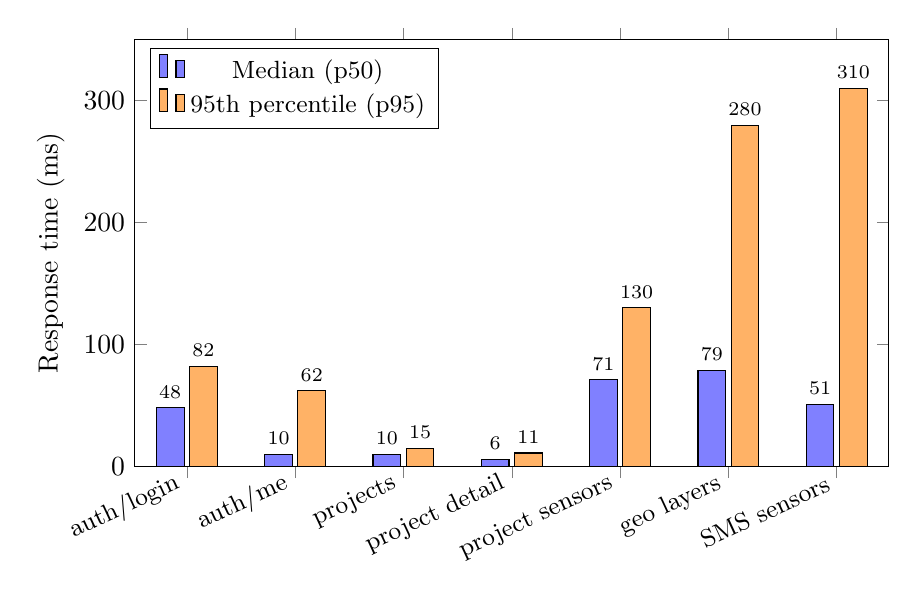
\begin{tikzpicture}
    \begin{axis}[
      ybar,
      bar width=10pt,
      width=0.92\textwidth,
      height=7cm,
      ylabel={Response time (ms)},
      symbolic x coords={auth/login, auth/me, projects, project detail,
                         project sensors, geo layers, SMS sensors},
      xtick=data,
      x tick label style={rotate=25, anchor=east, font=\small},
      ymin=0,
      ymax=350,
      enlarge x limits=0.08,
      legend style={at={(0.02,0.98)}, anchor=north west, font=\small},
      nodes near coords,
      every node near coord/.append style={font=\scriptsize},
    ]
    \addplot[fill=blue!50] coordinates {
      (auth/login, 48)
      (auth/me, 10)
      (projects, 10)
      (project detail, 6)
      (project sensors, 71)
      (geo layers, 79)
      (SMS sensors, 51)
    };
    \addplot[fill=orange!60] coordinates {
      (auth/login, 82)
      (auth/me, 62)
      (projects, 15)
      (project detail, 11)
      (project sensors, 130)
      (geo layers, 280)
      (SMS sensors, 310)
    };
    \legend{Median (p50), 95th percentile (p95)}
    \end{axis}
  \end{tikzpicture}
  \caption{API response time distribution under 10~concurrent users.
           Lightweight CRUD endpoints (projects, auth) respond within 15\,ms
           at p50. Data-heavy endpoints requiring FROST-Server fan-out (sensors,
           SMS) exhibit higher latency but remain well below the 2\,s threshold.}
  \label{fig:load-test-chart}
\end{figure}

\subsection{Time-Series Query Performance}
\label{sec:test-perf-timescaledb}

TimescaleDB partitions each per-thing observation table into time-based chunks. Time-range
queries, the dominant access pattern for chart rendering, benefit from chunk exclusion:
the query planner skips chunks outside the requested interval, reducing I/O to the relevant
time window. Older chunks are compressed automatically, further reducing storage requirements
and improving sequential scan throughput for historical queries.

Per-thing schema isolation provides an additional performance benefit: queries for one
sensor's data never scan another sensor's observation table, even when many sensors are
onboarded. This eliminates cross-sensor interference regardless of data volume.

\subsection{API Throughput}
\label{sec:test-perf-api}

Asynchronous request handlers with \texttt{httpx}-based FROST
client calls enable the FastAPI backend to serve multiple concurrent requests without blocking on
FROST-Server responses. The \texttt{AsyncFrostClient} maintains a connection pool
(100~maximum connections, 20~keep-alive) to reduce TCP handshake overhead for repeated
FROST queries. Under 10~concurrent users the backend sustains 4.9~requests/second
aggregate throughput; at 25~users this increases to 11.7~requests/second, confirming
near-linear scaling before the rate limiter constrains authentication-bound operations.

\clearpage
\subsection{Known Bottleneck}
\label{sec:test-perf-bottleneck}

The main performance bottleneck is the HTTP request fan-out to FROST-Server. Each
per-thing schema is served through its own FROST context path, so when the
the data platform API fetches sensor metadata for a project with many Things, it must
issue a separate HTTP request for each Thing. \texttt{AsyncThingService} mitigates
this by firing requests concurrently via \texttt{httpx} connection pooling, but the
fan-out pattern remains the throughput ceiling at scale. Adding a Redis caching layer
for frequently accessed metadata is a potential future optimization.

%% ----------------------------------------------------------------
\section{Deployment on CZU Infrastructure and eLTER Path}
\label{sec:test-deployment}
%% ----------------------------------------------------------------

On CZU infrastructure, the platform was deployed as the primary validation environment
for this thesis. This section documents the deployment, evaluates the platform's
readiness for adoption within the eLTER research infrastructure, and assesses the
long-term sustainability of the TSM-TEMP workarounds.

\subsection{CZU Deployment}
\label{sec:test-deployment-czu}

The deployment workflow described in Sections~\ref{sec:arch-deployment}
and~\ref{sec:impl-deploy} was validated on CZU infrastructure. The full stack of
22~containers was started using \texttt{make up}, with the post-deployment
\texttt{check.sh} script confirming container health, endpoint reachability across
all eight HTTP services, and credential consistency across the synchronised
\texttt{.env} variable pairs.

A platform audit conducted during this work identified and remediated 14~critical and
high-severity issues across the data platform codebase, including security header
enforcement, CORS and debug-mode controls, and credential management. An additional
27~issues were documented in the upstream TSM codebase, where remediation was not
feasible without upstream cooperation. The audit assessed all ten OWASP~Top~10
categories; accepted deferrals include the absence of a circuit-breaker pattern and
MQTT quality-of-service limited to level~1 by the upstream broker configuration.

At the time of writing, the deployment is live and publicly accessible at
\url{https://hydroportal-dev.dataraptors.eu}, where members of the CZU team are
actively accessing and evaluating the platform. This constitutes real-world validation
by the primary stakeholder group beyond automated tests and infrastructure smoke checks.

\subsection{Path to eLTER Adoption}
\label{sec:test-deployment-elter}

Several architectural properties of the platform align with eLTER requirements
described in Section~\ref{sec:bg-elter-implications}. The data access layer is built on the OGC
SensorThings API, which is a candidate standard for eLTER data exchange. Authentication
uses Keycloak with OpenID Connect, supporting the federated identity models common in
European research infrastructures. Project-based isolation provides the multi-tenancy
needed for hosting data from independent research sites. The containerized deployment
with single-file configuration enables reproducible installation across heterogeneous
institutional environments.

However, no eLTER-specific features have been implemented. The following gaps remain
between the current platform and a production-ready eLTER site-level deployment
(see Section~\ref{sec:bg-elter-ci} for the CI components referenced below):

\begin{itemize}
  \item \textbf{DEIMS-SDR site linkage.} The data model has no field for a DEIMS-SDR
    identifier, so observations cannot be linked to the eLTER site registry.
  \item \textbf{Vocabulary alignment.} Observed-property metadata is stored as
    free-text fields with no binding to EnvThes or eLTER Standard Observations.
  \item \textbf{DAR and OAR registration.} The platform cannot export metadata
    conforming to the eLTER dataset model, nor register the STA endpoint in the
    Online Asset Register.
  \item \textbf{eLTER~LogIn federation.} Keycloak would need to be configured as
    an identity broker for the eLTER~LogIn service (Perun~AAI).
  \item \textbf{Cross-site federation.} The platform operates as a single-site
    deployment; eLTER requires cross-site discovery and aggregated queries.
  \item \textbf{FAIR compliance.} Persistent identifiers (DOIs), provenance records,
    and machine-readable licensing metadata are absent.
\end{itemize}

These gaps are architectural and cannot be addressed by configuration changes
alone, but the foundational components (STA data access, OIDC authentication,
containerised deployment) are already in place for future work.

\subsection{Sustainability of the TSM-TEMP Workarounds}
\label{sec:test-deployment-tsmtemp}

The 18~\texttt{TSM-TEMP} marked locations in the codebase, concentrated in
\texttt{setup\_user\_database.py} and \texttt{sta\_views\_local/}, have shown no
operational disadvantages throughout the deployment period. The upstream SMS
service has remained non-functional throughout the duration of this thesis, and
no public roadmap for its restoration has been communicated. The assessment and
recommended migration path are discussed in
Section~\ref{sec:impl-tsm-assessment}.
